\documentclass{article}
\usepackage[utf8]{inputenc}
\usepackage{amsmath,amssymb}
\usepackage{paralist}
\usepackage{color}
\usepackage[detect-weight=true, binary-units=true]{siunitx}
\usepackage{pgfplots}
\usepackage{authblk}
\usepackage{url}
\usepackage{multirow}
\usepackage{booktabs}
\usepackage{graphicx}
\usepackage{float}
\usepackage{hyperref}
\title{Machine Learning and Data Mining project: leaf analysis}
\author{Guglielmo Padula}

\date{ AY $2021$-$2022$ - Data Science and Scientific Computing}



\begin{document}

\maketitle



\section{Problem statement}
The problem is to identify a leaf based on some of its attributes. 
The structure of the problem is the following:
\begin{itemize}
\item It takes as input  numerical vectors.
\item The output of the problem consists in a categorial variable.
\end{itemize}
The structure of the data is the following:
\begin{itemize}
\item the numerical vectors consists in the leaf attributes (length, height, ecc.)
\item the output categorical variable is the leaf name (a string)
\end{itemize}

\section{Proposed solution}
Based on the problem statement we want to solve a multiclassification problem. Specifically, we studied the performance of the following techniques:
\begin{itemize}
\item Bayes classifier
\item K nearest neightbours classifier
\item SVM classifier
\item Random Forest classifier
\end{itemize}

\section{Assessment and performance indexes}
To assess the validity of the procedure I use two performance indexes:
\begin{itemize}
\item the missclassification error rate 
\item the AUC index
\end{itemize}
The AUC index is also considered so we can assess quality also in presence on unbalanced data. The AUC index is defined only for binay classification case. We apply it to multiclass classification in the following way: we measure the AUC for every single class taking it as positive (one vs all approach) and then we take the average.\\
These two indexes are estimated on both the training set and on the test set.


\section{Experimental evaluation}

\subsection{Data}
The full dataset that I used for studying the problem is avaiable  here: \url{ https://archive.ics.uci.edu/ml/machine-learning-databases/00288/}.
It contains data about 40 different plant species, however only 30 species have numerical data. The data of the others will be discarded. There is also a feature regarding the implict ordering of the observations, which has no informative content, so it will be discarded.  What remains of data is composed of $n=340$ observations with $p=14$ numerical features (the attributes of the leaf) and a categorial variable (the label of the leaf).  The data is unbalanced.  


\subsection{Specific setup for each technique}
\subsubsection{Bayes classifier}
We to use the naive bayes classifier, because we can assume that the features are independent.
\subsubsection{KNN classifier}
About the Knn classifier we considered  $k$ implicit based on the minimization of the $10CV$ error on the training data.  

\subsection{Random Forest classifier}
For the Random Forest classifier we tested different values of $mtry (1,2,3,4,5)$  and to the choice of $B$ implicit  based on the minimization of the $10CV$ error on the training data.\\
The following image shows the 10CV errov with respect to $B$ and $mtry$.\\
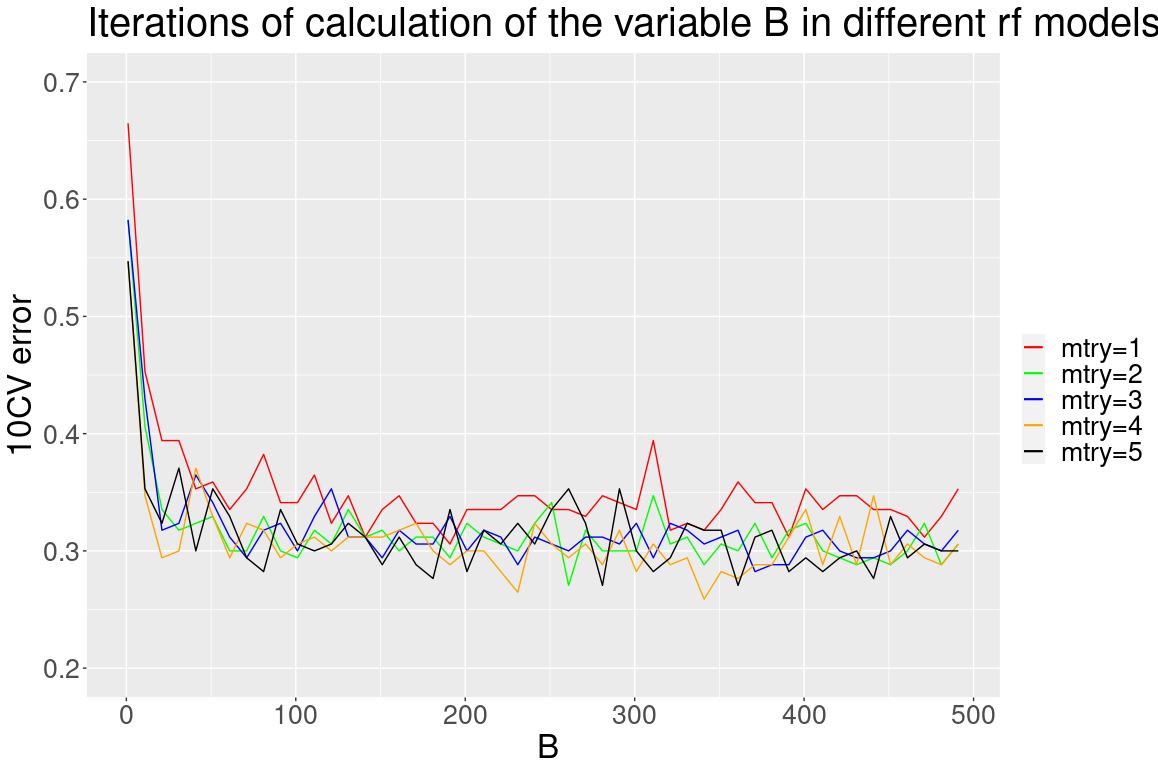
\includegraphics[scale=0.30]{rf}

\subsection{SVM}
For the SVM classifier we tested multiple kernels with different parameters, with the choice of $C$  based on the minimization of the $10CV$ error on the training data. The following combinations have been tested:
\begin{itemize}
\item Radial kernel with gamma=0.1,0.6,1.1,1.6,2.1
\item Sigmoid kernel with gamma=0.1,0.6,1.1,1.6,2.1
\item Linear kernel 
\item polynomial kernel with degree 2 or 3
\end{itemize}
The following image shows the 10CV errov with respect to $C$ and the various combinations of gamma and kernel tested.\\
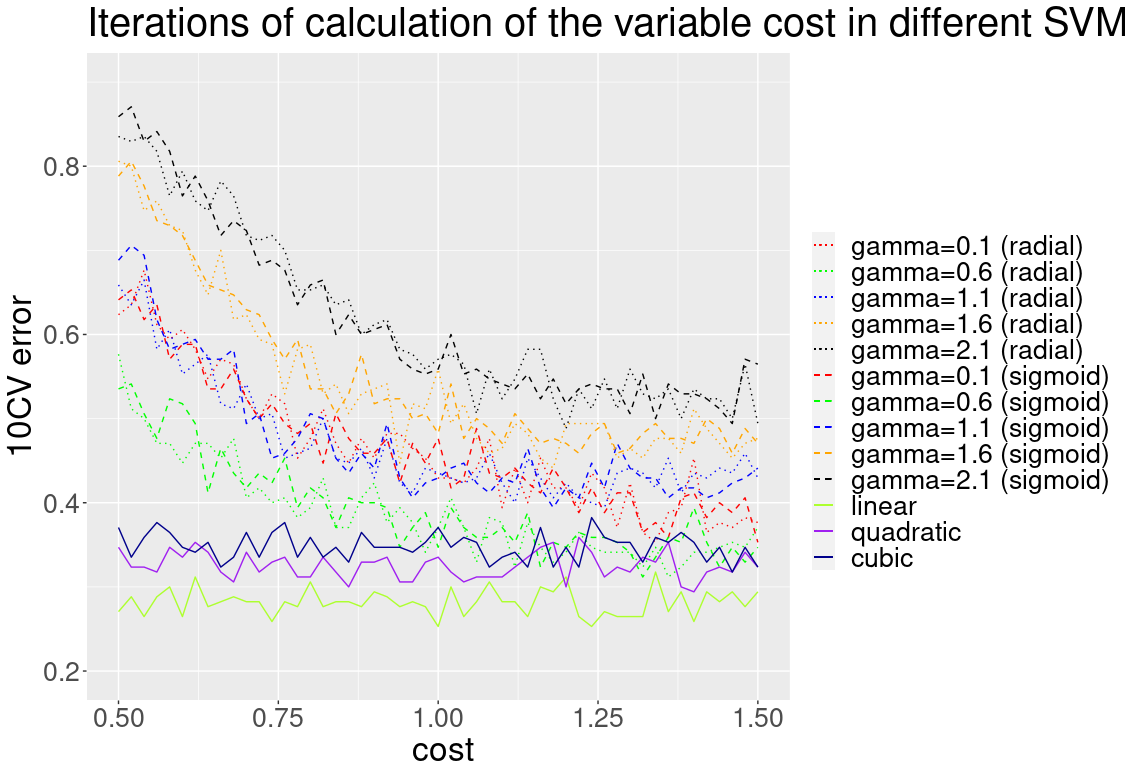
\includegraphics[scale=0.30]{svm}
\\
\subsection{Results and discussion}
We use a random classifier as a baseline.
Follows a table of the performances of every model tested.
\\
\begin{table}[H]
\begin{tabular}{lllll}
                         & training error rate & training AUC & test error rate & test AUC \\
RF (mtry=1)              & 0                   & 1            & 0.23            & 0.89     \\
RF (mtry=2)              & 0                   & 1            & 0.24            & 0.88     \\
RF (mtry=3)              & 0                   & 1            & 0.24            & 0.87     \\
RF (mtry=4)              & 0                   & 1            & 0.25            & 0.87     \\
RF(mtry=5)               & 0                   & 1            & 0.25            & 0.86     \\
Naive bayes              & 0.14                & 0.93         & 0.32            & 0.84     \\
Knn                      & 0                   & 1            & 0.29            & 0.78     \\
Radial svm (gamma=0.1)   & 0.23                & 0.88         & 0.31            & 0.83     \\
Radial svm (gamma=0.6)   & 0.08                & 0.96         & 0.32            & 0.84     \\
Radial svm (gamma=1.1)   & 0.03                & 0.98         & 0.39            & 0.79     \\
Radial svm (gamma=1.6)   & 0.02                & 0.99         & 0.44            & 0.76     \\
Radial svm (gamma=2.1)   & 0.02                & 0.99         & 0.49            & 0.73     \\
Sigmoid svm (gamma=0.1) & 0.59                & 0.68         & 0.69            & 0.63     \\
Sigmoid svm (gamma=0.6) & 0.86                & 0.54         & 0.86            & 0.54     \\
Sigmoid svm (gamma=1.1) & 0.88                & 0.53         & 0.89            & 0.53     \\
Sigmoid svm (gamma=1.6) & 0.87                & 0.54         & 0.89            & 0.53     \\
Sigmoid svm (gamma=2.1) & 0.87                & 0.54         & 0.89            & 0.53     \\
Linear svm               & 0.11                & 0.94         & 0.27            & 0.71     \\
Quadratic svm            & 0.0132              & 0.99         & 0.27            & 0.86     \\
Cubic svm                & 0                   & 1            & 0.27            & 0.85     \\
Random classifier        & 0.97                & 0.50          & 0.95            & 0.51     
\end{tabular}
\end{table}
Our ideal objective is to maximize the test AUC and minimize the test error, so the best classifier is RF with mtry=1, which significantly surpass the random classifier.  About the radial and sigmoid svm classifier, with the increasing of gamma there is a behaviour of increasing overfitting.


\bibliographystyle{plain}
\bibliography{bibliography}

\end{document}
